\begin{figure*}
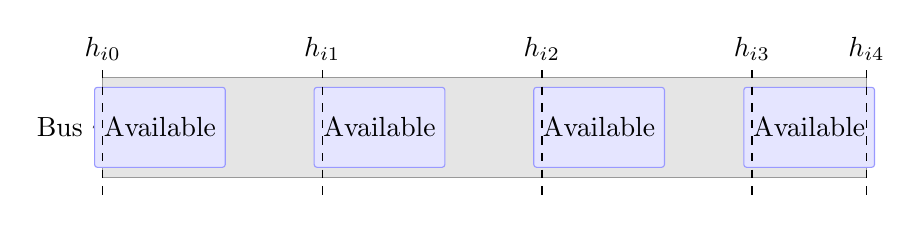
\begin{tikzpicture}
\node[rectangle, draw=black!40, fill=black!10, minimum width=0.8\textwidth, minimum height=0.5in](charger1Box) at (0.5\textwidth,1){};
	\node(bus1BoxLabel) at (0.065\textwidth, 1){Bus $i$}; 
	\node[rectangle, draw=blue!40, fill=blue!10, minimum width=0.12\textwidth, minimum height=0.4in, rounded corners=1pt] at (0.16\textwidth,1){Available};
	\node[rectangle, draw=blue!40, fill=blue!10, minimum width=0.12\textwidth, minimum height=0.4in, rounded corners=1pt] at (0.39\textwidth,1){Available};
	\node[rectangle, draw=blue!40, fill=blue!10, minimum width=0.12\textwidth, minimum height=0.4in, rounded corners=1pt] at (0.62\textwidth,1){Available};
	\node[rectangle, draw=blue!40, fill=blue!10, minimum width=0.12\textwidth, minimum height=0.4in, rounded corners=1pt] at (0.84\textwidth,1){Available};

	\node(h0High) at (0.1\textwidth,2){$h_{i0}$};
	\node(h0Low) at (0.1\textwidth,0.05){};
	\draw[dashed, line width=0.5pt] (h0High) -- (h0Low.center);

	\node(h1High) at (0.33\textwidth,2){$h_{i1}$};
	\node(h1Low) at (0.33\textwidth,0.05){};
	\draw[dashed, line width=0.5pt] (h1High) -- (h1Low.center);

	\node(h0High) at (0.56\textwidth,2){$h_{i2}$};
	\node(h0Low) at (0.56\textwidth,0.05){};
	\draw[dashed, line width=0.5pt] (h0High) -- (h0Low.center);

	\node(h0High) at (0.78\textwidth,2){$h_{i3}$};
	\node(h0Low) at (0.78\textwidth,0.05){};
	\draw[dashed, line width=0.5pt] (h0High) -- (h0Low.center);

	\node(h0High) at (0.9\textwidth,2){$h_{i4}$};
	\node(h0Low) at (0.9\textwidth,0.05){};
	\draw[dashed, line width=0.5pt] (h0High) -- (h0Low.center);
\end{tikzpicture}
\caption{State of Charge Variables}
\label{fig:hPlacement}
\end{figure*}
